\documentclass[journal,12pt,twocolumn]{IEEEtran}

\usepackage{setspace}
\usepackage{gensymb}

\singlespacing


\usepackage[cmex10]{amsmath}

\usepackage{amsthm}

\usepackage{mathrsfs}
\usepackage{txfonts}
\usepackage{stfloats}
\usepackage{bm}
\usepackage{cite}
\usepackage{cases}
\usepackage{subfig}

\usepackage{longtable}
\usepackage{multirow}

\usepackage{enumitem}
\usepackage{mathtools}
\usepackage{steinmetz}
\usepackage{tikz}
\usepackage{circuitikz}
\usepackage{verbatim}
\usepackage{tfrupee}
\usepackage[breaklinks=true]{hyperref}
\usepackage{graphicx}
\usepackage{tkz-euclide}

\usetikzlibrary{calc,math}
\usepackage{listings}
    \usepackage{color}                                            %%
    \usepackage{array}                                            %%
    \usepackage{longtable}                                        %%
    \usepackage{calc}                                             %%
    \usepackage{multirow}                                         %%
    \usepackage{hhline}                                           %%
    \usepackage{ifthen}                                           %%
    \usepackage{lscape}     
\usepackage{multicol}
\usepackage{chngcntr}

\DeclareMathOperator*{\Res}{Res}

\renewcommand\thesection{\arabic{section}}
\renewcommand\thesubsection{\thesection.\arabic{subsection}}
\renewcommand\thesubsubsection{\thesubsection.\arabic{subsubsection}}

\renewcommand\thesectiondis{\arabic{section}}
\renewcommand\thesubsectiondis{\thesectiondis.\arabic{subsection}}
\renewcommand\thesubsubsectiondis{\thesubsectiondis.\arabic{subsubsection}}


\hyphenation{op-tical net-works semi-conduc-tor}
\def\inputGnumericTable{}                                 %%

\lstset{
%language=C,
frame=single, 
breaklines=true,
columns=fullflexible
}
\begin{document}


\newtheorem{theorem}{Theorem}[section]
\newtheorem{problem}{Problem}
\newtheorem{proposition}{Proposition}[section]
\newtheorem{lemma}{Lemma}[section]
\newtheorem{corollary}[theorem]{Corollary}
\newtheorem{example}{Example}[section]
\newtheorem{definition}[problem]{Definition}

\newcommand{\BEQA}{\begin{eqnarray}}
\newcommand{\EEQA}{\end{eqnarray}}
\newcommand{\define}{\stackrel{\triangle}{=}}
\bibliographystyle{IEEEtran}

\providecommand{\mbf}{\mathbf}
\providecommand{\pr}[1]{\ensuremath{\Pr\left(#1\right)}}
\providecommand{\qfunc}[1]{\ensuremath{Q\left(#1\right)}}
\providecommand{\sbrak}[1]{\ensuremath{{}\left[#1\right]}}
\providecommand{\lsbrak}[1]{\ensuremath{{}\left[#1\right.}}
\providecommand{\rsbrak}[1]{\ensuremath{{}\left.#1\right]}}
\providecommand{\brak}[1]{\ensuremath{\left(#1\right)}}
\providecommand{\lbrak}[1]{\ensuremath{\left(#1\right.}}
\providecommand{\rbrak}[1]{\ensuremath{\left.#1\right)}}
\providecommand{\cbrak}[1]{\ensuremath{\left\{#1\right\}}}
\providecommand{\lcbrak}[1]{\ensuremath{\left\{#1\right.}}
\providecommand{\rcbrak}[1]{\ensuremath{\left.#1\right\}}}
\theoremstyle{remark}
\newtheorem{rem}{Remark}
\newcommand{\sgn}{\mathop{\mathrm{sgn}}}
\providecommand{\abs}[1]{\left\vert#1\right\vert}
\providecommand{\res}[1]{\Res\displaylimits_{#1}} 
\providecommand{\norm}[1]{\left\lVert#1\right\rVert}
%\providecommand{\norm}[1]{\lVert#1\rVert}
\providecommand{\mtx}[1]{\mathbf{#1}}
\providecommand{\mean}[1]{E\left[ #1 \right]}
\providecommand{\fourier}{\overset{\mathcal{F}}{ \rightleftharpoons}}
%\providecommand{\hilbert}{\overset{\mathcal{H}}{ \rightleftharpoons}}
\providecommand{\system}{\overset{\mathcal{H}}{ \longleftrightarrow}}
	%\newcommand{\solution}[2]{\textbf{Solution:}{#1}}
\newcommand{\solution}{\noindent \textbf{Solution: }}
\newcommand{\cosec}{\,\text{cosec}\,}
\providecommand{\dec}[2]{\ensuremath{\overset{#1}{\underset{#2}{\gtrless}}}}
\newcommand{\myvec}[1]{\ensuremath{\begin{pmatrix}#1\end{pmatrix}}}
\newcommand{\mydet}[1]{\ensuremath{\begin{vmatrix}#1\end{vmatrix}}}

\numberwithin{equation}{subsection}

\makeatletter
\@addtoreset{figure}{problem}
\makeatother
\let\StandardTheFigure\thefigure
\let\vec\mathbf

\renewcommand{\thefigure}{\theproblem}

\def\putbox#1#2#3{\makebox[0in][l]{\makebox[#1][l]{}\raisebox{\baselineskip}[0in][0in]{\raisebox{#2}[0in][0in]{#3}}}}
     \def\rightbox#1{\makebox[0in][r]{#1}}
     \def\centbox#1{\makebox[0in]{#1}}
     \def\topbox#1{\raisebox{-\baselineskip}[0in][0in]{#1}}
     \def\midbox#1{\raisebox{-0.5\baselineskip}[0in][0in]{#1}}
\vspace{3cm}
\title{Assignment 1}
\author{Kusuma Priya}

\maketitle
\newpage

\bigskip
\renewcommand{\thefigure}{\theenumi}
\renewcommand{\thetable}{\theenumi}
Download all python codes from 
\begin{lstlisting}
https://github.com/KUSUMAPRIYAPULAVARTY/assignment1/tree/master/codes
\end{lstlisting}
%
and latex-tikz codes from 
%
\begin{lstlisting}
https://github.com/KUSUMAPRIYAPULAVARTY/assignment1
\end{lstlisting}
%
 
 \section{Question No. 40}
Two lines passing through the point \myvec{2\\3} intersect each other at an angle of 60\degree. If one line has slope 2, find equation of the other line. 
%

\section{Explanation}
Directional vector of a line having slope 2 is \myvec{1\\2}
Hence normal vector n$_1$ is given as
\begin{align}
n_1 =\myvec{0 & -1\\1 & 0}\myvec{1\\2}\\=\myvec{-2\\1}
\end{align}
Similarly normal vector for line 2 \\
\begin{align}
n_2 = \myvec{-m_2\\1}
\end{align}
Angle between two lines $\theta$ can be given by

\begin{align}
\cos \theta &= \frac{\vec{n_1}^T\vec{n_2}}{\norm{\vec{n_1}}\norm{\vec{n_2}}}\\
\implies \cos 60\degree &=\frac{1}{2}\\ 
=\frac{2m_2+1}{\sqrt5\times\sqrt{1+m_2}}
\end{align}
 \begin{align}
 \implies 11m_2^2+16m_2-1=0
 \end{align}
 Solving, m$_2$ yields values $\frac{-8+5\sqrt{3}}{11}$ and $\frac{-8-5\sqrt{3}}{11}$ \\
 Equation of line with normal vector\vec{n} and passing through point A is given by
 \begin{align}
 \vec{n}^T(\vec{X}-A)=0
 \end{align}
  Hence,equation of line with slope $\frac{-8+5\sqrt{3}}{11}$ passing through \myvec{2\\3} is
  \begin{align}
  \myvec{\frac{8-5\sqrt{3}}{11}&1}\left(\vec{X}-\myvec{2\\3}\right)=0\\
  \implies \myvec{\frac{8-5\sqrt{3}}{11}&1}\vec{X}=\frac{49-10\sqrt{3}}{11}
  \end{align}
  Similarly,equation of line with slope $\frac{-8-5\sqrt{3}}{11}$ passing through \myvec{2\\3} is
  \begin{align}
  \myvec{\frac{8+5\sqrt{3}}{11}&1}\left(\vec{X}-\myvec{2\\3}\right)=0\\
  \implies \myvec{\frac{8+5\sqrt{3}}{11}&1}\vec{X}=\frac{49+10\sqrt{3}}{11}
  \end{align}
  Thus, the required line equations are
  \begin{align}
  \myvec{\frac{8-5\sqrt{3}}{11}&1}\vec{X}=\frac{49-10\sqrt{3}}{11} 
  \end{align}
  \begin{align}
  and
  \end{align}
  \begin{align}
   \myvec{\frac{8+5\sqrt{3}}{11}&1}\vec{X}=\frac{49+10\sqrt{3}}{11}
  \end{align}
  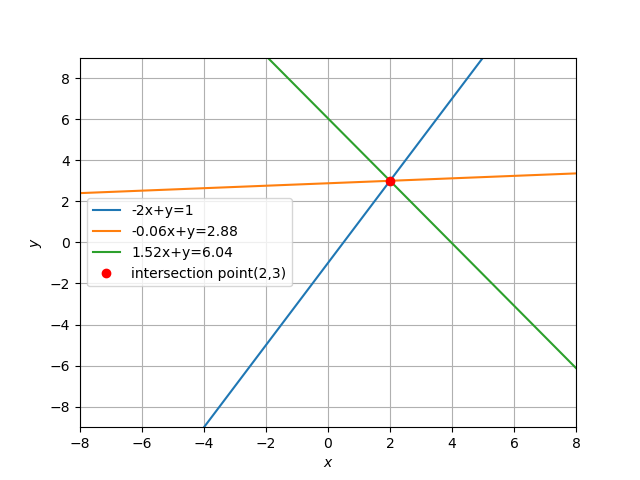
\includegraphics{plot.png}
\end{document}
